%%%%%%%%%%%%%%%%%%%%%%%%%%%%%%%%%%%%%%%%%%%%%%%%%%%%%%%%%%%%%%%%%%%%%%%%%%%%%%%%%%%%%
%% Template LaTeX de Proposta de Monografia do Departamento de Sistemas de          %
%% Informação (DSI) da Universidade Federal de Sergipe (UFS)                        %
%% Elaborado por Breno Santana Santos (http://brenosantos.bssystems.com.br).        %
%%%%%%%%%%%%%%%%%%%%%%%%%%%%%%%%%%%%%%%%%%%%%%%%%%%%%%%%%%%%%%%%%%%%%%%%%%%%%%%%%%%%%
\documentclass{dsi-tcc1}

%%%%%%%%%%%%%%%%%%%%%%%%%%%%%%%%%%%%%%%%%%%%%%%%%%%%%%%%%%%%%%%%%%%%%%%%%%%%%%%
% Observação: Remover esse pacote e o texto gerado por ele no momento da
% confecção da versão da proposta.
% Geração de texto de exemplo.
\usepackage{lipsum}
%%%%%%%%%%%%%%%%%%%%%%%%%%%%%%%%%%%%%%%%%%%%%%%%%%%%%%%%%%%%%%%%%%%%%%%%%%%%%%%

%%%%%%%%%%%%%%%%%%%%%%%%%%%%%%%%%%%%%%%%%%%%%%%%%%%%%%%%%%%%%%%%%%%%%%
\universidade{Universidade Federal de Sergipe}
\centroCampus{Campus Prof. Alberto Carvalho}
\departamento{Departamento de Sistemas de Informação}
\titulo{Preencher com o Título da Proposta}
\orientador{Prof. Preencher}
% Descomente a linha abaixo, caso haja um professor co-orientador.
% \coorientador{Prof. Preencher}
\aluno{Preencher}
%%%%%%%%%%%%%%%%%%%%%%%%%%%%%%%%%%%%%%%%%%%%%%%%%%%%%%%%%%%%%%%%%%%%%%

\begin{document}
   % Cabeçalho.
    \cabecalho

    % Conteúdo.
	\section{Introdução}\label{sec:intro}

A introdução é uma parte fundamental de qualquer trabalho acadêmico. Ela serve como uma porta de entrada para o leitor, oferecendo uma visão geral do tema e preparando-o para o conteúdo que será discutido ao longo do trabalho \cite{Marconi2021}. A introdução deve capturar o interesse do leitor e fornecer informações suficientes para que ele entenda o contexto e a relevância do estudo \cite{Wazlawick2021}.

Segundo \citeonline{Marconi2022}, os principais elementos e objetivos de uma introdução são:
\begin{enumerate}[label=\alph*), itemsep=0pt, leftmargin=2.5cm]
    \item \textbf{Abertura:} um parágrafo inicial que introduz o tema de forma ampla e instigante, capturando o interesse do leitor.
    \item \textbf{Contextualização:} apresentar o tema de maneira geral --- uma explicação mais detalhada do tema ---, situando o leitor no contexto em que a pesquisa está inserida. Isso pode incluir uma breve revisão da literatura, destacando trabalhos relevantes e mostrando como o seu trabalho se encaixa nesse contexto.
    \item \textbf{Justificativa e Relevância:} explicar a relevância do tema, a importância e contribuição do trabalho para o campo de estudo. Isso pode envolver a apre\-sentação de lacunas na literatura existente ou problemas práticos que a pesquisa pretende abordar.
    \item \textbf{Problema de Pesquisa:} apresentar claramente o problema de pesquisa que o trabalho pretende resolver. O problema de pesquisa deve ser formulado de maneira clara, precisa e concisa.
    \item \textbf{Hipóteses (opcional):} em alguns tipos de pesquisa, especialmente aquelas de caráter experimental, é importante apresentar as hipóteses que serão testadas, se aplicável.
\end{enumerate}

Desse modo, a introdução é crucial para estabelecer o cenário do trabalho e orientar o leitor sobre o que esperar nas seções seguintes. É de suma importância o pesquisador ser claro, conciso e informativo para garantir que o leitor compreenda a relevância do seu estudo desde o início.
    \section{Objetivos do Projeto}\label{sec:obj_proj}

Esta seção é responsável por descrever os objetivos da proposta. Dessa forma, os objetivos devem ser definidos de forma a orientar o leitor sobre o que se pretende alcançar com o estudo \cite{Marconi2021}. Em geral, essa seção inicia-se com um parágrafo da seguinte forma:

\textit{Para a realização deste estudo, têm-se os seguintes objetivos geral e específicos.}

\subsection{Objetivo Geral}

O objetivo geral é uma declaração ampla que descreve a meta principal do seu trabalho acadêmico ou de pesquisa. Ele indica o propósito/contribuição central do estudo e o que você espera alcançar de maneira abrangente. O objetivo geral é mais amplo e menos específico do que os objetivos específicos \cite{Marconi2021,Wazlawick2021}.

Em geral, inicia-se um objetivo geral da seguinte forma: \textit{O presente projeto tem como objetivo geral...}

De acordo com \citeonline{Marconi2022}, as principais características de um objetivo geral são:
\begin{itemize}[itemsep=0pt, leftmargin=2.5cm]
    \item \textbf{Amplo e Abrangente:} ele cobre a essência da pesquisa de maneira ampla, sem entrar em detalhes específicos, e explica por que isso é relevante.
    \item \textbf{Claro e Conciso:} deve ser formulado de maneira clara e direta, facilitando o entendimento do propósito/contribuição do estudo.
    \item \textbf{Alinhado com o Problema de Pesquisa:} deve estar diretamente relacionado ao problema de pesquisa que você está abordando.
    \item \textbf{Orientador:} fornece uma direção clara para orientar toda a pesquisa, ajudando a manter o foco no propósito central do estudo, ao longo do desenvolvimento do trabalho.
    \item \textbf{Guia a Estrutura do Trabalho:} ajuda a orientar a estrutura do trabalho, influenciando a formulação dos objetivos específicos, a metodologia e as conclusões.
\end{itemize}

Ao formular o objetivo geral, é importante que ele seja realista e alcançável dentro do escopo e das limitações do seu estudo. Ele deve proporcionar uma visão clara do propósito do seu trabalho e preparar o terreno para a definição dos objetivos específicos \cite{Marconi2021}.

\subsection{Objetivos Específicos}\label{sec:obj_proj_esp}

Por sua vez, os objetivos específicos são declarações detalhadas e concretas que descrevem as etapas ou metas menores que precisam ser alcançadas para que o objetivo geral do trabalho acadêmico ou de pesquisa seja atingido. Ou seja, representam subprodutos do objetivo geral e, consequentemente, do trabalho em si \cite{Wazlawick2021}. Em síntese, eles desmembram o objetivo geral em partes mais manejáveis e operacionais, fornecendo um guia claro para o desenvolvimento do estudo.

Em geral, os objetivos específicos podem ser definidos da seguinte forma:

\textit{Os objetivos específicos, componentes do objetivo geral, são:}
\begin{enumerate}[label=\textit{\alph*)}, itemsep=0pt, leftmargin=2.5cm]
    \item \textit{Objetivo Específico 01...}
    \item \textit{Objetivo Específico 02...}
\end{enumerate}

Conforme \citeonline{Marconi2021}, e \citeonline{Wazlawick2021} destacam, as principais características dos objetivos específicos são:
\begin{itemize}[itemsep=0pt, leftmargin=2.5cm]
    \item \textbf{Detalhados e Precisos:} devem ser claramente definidos e específicos, indicando exatamente o que será investigado ou realizado, além de proporcionar um plano claro para a condução da pesquisa.
    \item \textbf{Mensuráveis:} é importante que sejam mensuráveis ou verificáveis, permitindo avaliar se foram alcançados. Também permitem monitorar o progresso do estudo, verificando se cada etapa está sendo cumprida conforme planejado.
    \item \textbf{Atingíveis:} devem ser realistas e alcançáveis dentro do escopo do estudo.
    \item \textbf{Relevantes:} cada objetivo específico deve contribuir diretamente para o alcance do objetivo geral.
    \item \textbf{Temporais:} quando aplicável, podem incluir um prazo para serem alcançados.
    \item \textbf{Orientação Metodológica:} guiam a escolha dos métodos e procedimentos a serem utilizados para a coleta e análise de dados.
    \item \textbf{Clareza e Foco:} mantêm o foco do pesquisador no que é realmente importante para alcançar o objetivo geral, evitando desvios desnecessários.
\end{itemize}

Geralmente, os objetivos específicos começam com verbos de ação que indicam claramente o que será feito. Seguem alguns exemplos de verbos frequentemente usados: analisar, investigar, identificar, avaliar, descrever, comparar, determinar, medir, testar, verificar, entre outros.

Por fim, eles são essenciais para guiar o desenvolvimento e a execução de um trabalho acadêmico, garantindo que cada etapa seja bem definida e contribua para a realização do objetivo geral.
    \section{Revisão Bibliográfica Inicial}\label{sec:revisao_bib}

A revisão bibliográfica é uma seção crucial de um trabalho acadêmico ou científico que fornece a base teórica e conceitual sobre a qual a pesquisa é construída. Ela consiste na exposição e discussão das teorias, modelos, conceitos e estudos relevantes que sustentam e orientam a investigação proposta \cite{Marconi2022}.

Conforme \citeonline{Wazlawick2021} enfatiza, seus objetivos são:
\begin{itemize}[itemsep=0pt, leftmargin=2.5cm]
    \item \textbf{Fundamentar a Pesquisa:} oferecer uma base teórica sólida que justifica e sustenta a pesquisa, demonstrando o entendimento do pesquisador sobre o tema.
    \item \textbf{Definir Conceitos:} clarificar os conceitos e termos chave utilizados no estudo, garantindo que todos os leitores compreendam os significados específicos adotados e evitando ambiguidades.
    \item \textbf{Enquadrar o Problema:} situar o problema de pesquisa dentro de um contexto teórico mais amplo, mostrando como ele se relaciona com o conhecimento existente.
    \item \textbf{Orientar a Metodologia:} fundamentar a escolha dos métodos e técnicas de pesquisa, com base em abordagens teóricas consagradas.
    \item \textbf{Interpretar Resultados:} oferecer uma lente teórica através da qual os dados coletados serão analisados e interpretados, favorecendo a discussão dos resultados.
\end{itemize}

Ademais, de acordo com \citeonline{Marconi2021}, sua estrutura pode variar dependendo do campo de estudo e do tipo de pesquisa, mas geralmente inclui os seguintes componentes:
\begin{enumerate}[label=\roman*., itemsep=0pt, leftmargin=2.5cm]
    \item \textbf{Introdução:} apresenta a importância da revisão bibliográfica e como ela está organizada.
    \item \textbf{Revisão de Teorias e Modelos Relevantes:}
        \begin{itemize}
            \item \textbf{Principais Teorias:} discussão das principais teorias que sustentam o estudo. Isso pode incluir teorias clássicas e contemporâneas.
            \item \textbf{Modelos Conceituais:} apresentação de modelos conceituais que serão utilizados para entender e analisar o problema de pesquisa.
        \end{itemize}
    \item \textbf{Discussão de Conceitos-Chave:}
        \begin{itemize}
            \item \textbf{Definição de Conceitos:} definição e discussão detalhada dos conceitos principais utilizados no estudo.
            \item \textbf{Aplicabilidade dos Conceitos:} explicação de como esses conceitos serão aplicados na pesquisa.
        \end{itemize}
    \item \textbf{Revisão de Estudos Empíricos:} síntese dos estudos empíricos relevantes que utilizaram as teorias e conceitos discutidos, mostrando como eles foram aplicados e os resultados obtidos. Conhecida como trabalhos relacionados/correlatos.
    \item \textbf{Conclusão:} resumo do referencial teórico, destacando como ele sustenta a pesquisa e preparando o terreno para a metodologia.
\end{enumerate}

Desse modo, \citeonline{Marconi2022} afirmam que os passos para realizar uma revisão bibliográfica são:
\begin{enumerate}[label=\roman*., itemsep=0pt, leftmargin=2.5cm]
    \item \textbf{Levantamento Bibliográfico:} realizar uma revisão extensiva da literatura para identificar teorias, modelos e estudos relevantes.
    \item \textbf{Seleção de Fontes:} selecionar as fontes mais pertinentes e de alta qualidade para incluir na revisão bibliográfica.
    \item \textbf{Organização do Conteúdo:} estruturar o conteúdo de forma lógica e coerente, agrupando as teorias e conceitos de maneira que façam sentido e sustentem a pesquisa.
    \item \textbf{Escrita Crítica:} redigir a seção de forma crítica, não apenas descrevendo as teorias e estudos, mas também discutindo suas implicações, limitações e relevância para a pesquisa.
    \item \textbf{Integração com a Pesquisa:} garantir que a revisão bibliográfica esteja diretamente ligada ao problema de pesquisa e aos objetivos do estudo, demonstrando claramente como ela fundamenta e orienta a investigação.
\end{enumerate}

Portanto, a revisão bibliográfica é uma seção indispensável que confere rigor e credibilidade a um trabalho acadêmico, estabelecendo uma base sólida para a condução e interpretação da pesquisa.

\subsection{Trabalhos Correlatos}

A seção de trabalhos relacionados, também conhecida como revisão da literatura, estudos correlatos ou estado da arte, é uma parte essencial de um trabalho acadêmico ou científico. Trata-se de uma análise crítica e síntese das pesquisas e publicações já existentes sobre um determinado tema \cite{Marconi2021}. Ou seja, tem como objetivo revisar, comparar e contrastar os estudos e pesquisas anteriores que são relevantes para o tema em investigação.

Dessa forma, seu foco principal é proporcionar uma compreensão profunda e abrangente do estado atual do conhecimento sobre o assunto, identificar lacunas na pesquisa existente, e estabelecer um contexto teórico e metodológico para o estudo em questão. Ela também ajuda a situar o seu trabalho dentro do contexto existente de conhecimento, destacando como ele se relaciona com outras pesquisas na área \cite{Wazlawick2021}.

Assim, conforme \citeonline{Marconi2022} destacam, seus objetivos são:
\begin{itemize}[itemsep=0pt, leftmargin=2.5cm]
    \item \textbf{Contextualizar a Pesquisa:} situar o estudo dentro do corpo existente de conhecimento, mostrando a relevância e a contribuição da pesquisa proposta. Em síntese, oferece uma base de conhecimento que sustenta a pesquisa.
    \item \textbf{Identificar Lacunas:} revelar áreas onde há falta de informação ou, em que a pesquisa é insuficiente, justificando a necessidade do novo estudo.
    \item \textbf{Comparar Metodologias e Resultados:} comparar as metodologias e os resultados de estudos anteriores com os seus, destacando similaridades e diferenças.
    \item \textbf{Fundamentar a Pesquisa:} oferecer uma base sólida para a escolha da metodologia e para a interpretação dos resultados do seu estudo.
    \item \textbf{Evitar Redundâncias:} garantir que o estudo não repita trabalhos já existentes sem contribuir com algo novo. Portanto, garante que a pesquisa contribua de maneira nova e significativa para o campo.
\end{itemize}

Além disso, \citeonline{Wazlawick2021} complementa que a estrutura de uma seção de trabalhos correlatos pode variar dependendo do campo de estudo e do tipo de pesquisa, mas geralmente inclui os seguintes componentes:
\begin{enumerate}[label=\roman*., itemsep=0pt, leftmargin=2.5cm]
    \item \textbf{Introdução:} apresenta o propósito da seção e explica como ela está organizada.
    \item \textbf{Revisão de Trabalhos Anteriores:}
        \begin{itemize}
            \item \textbf{Organização Temática:} eles podem ser agrupados por temas, tópicos ou questões de pesquisa.
            \item \textbf{Organização Cronológica:} eles podem ser apresentados em ordem cronológica para mostrar a evolução da pesquisa no campo.
            \item \textbf{Organização Metodológica:} eles podem ser agrupados de acordo com as metodologias utilizadas.
        \end{itemize}
    \item \textbf{Discussão Crítica:}
        \begin{itemize}
            \item \textbf{Análise Comparativa:} comparar e contrastar os resultados, metodologias e abordagens dos estudos revisados.
            \item \textbf{Identificação de Lacunas:} destacar onde os estudos anteriores falham ou onde há oportunidades para novas pesquisas.
            \item \textbf{Relação com sua Pesquisa:} explicar como os estudos anteriores influenciam ou justificam sua pesquisa.
        \end{itemize}
    \item \textbf{Conclusão:} resumir os principais pontos discutidos na seção, destacando as lacunas identificadas e preparando o terreno para a apresentação do seu estudo.
\end{enumerate}

Outrossim, conforme \citeonline{Marconi2022} explanam, os passos para elaborar uma seção de trabalhos relacionados são:
\begin{enumerate}[label=\roman*., itemsep=0pt, leftmargin=2.5cm]
    \item \textbf{Levantamento Bibliográfico:} realize uma busca extensa nas bases de dados acadêmicas para identificar os estudos relevantes.
    \item \textbf{Seleção de Fontes:} selecione os trabalhos mais pertinentes e de alta qualidade para incluir na seção. Para isso, utilize bases de dados acadêmicas, bibliotecas, revistas científicas e outras fontes relevantes para encontrar artigos, livros, teses e outros materiais pertinentes.
    \item \textbf{Leitura Crítica:} leia os estudos selecionados de forma crítica, avaliando suas metodologias, resultados e relevância.
    \item \textbf{Organização do Conteúdo:} estruture a seção de maneira lógica e coerente, agrupando os estudos de acordo com temas, cronologia ou metodologia.
    \item \textbf{Redação Crítica:} redija a seção de maneira crítica e analítica, não apenas descrevendo os estudos, mas discutindo suas contribuições, limitações e relação com sua pesquisa. Ou seja, faça uma síntese das principais descobertas, destacando semelhanças e diferenças entre os estudos.
    \item \textbf{Integração com seu Trabalho:} relacione os estudos revisados com sua própria pesquisa, mostrando como eles influenciam sua abordagem e justificam a necessidade do seu estudo.
\end{enumerate}

Portanto, a seção de trabalhos relacionados é essencial para estabelecer a relevância e originalidade da sua pesquisa, oferecendo um panorama detalhado do conhecimento existente e preparando o terreno para a sua contribuição específica ao campo de estudo.
    \section{Metodologia}\label{sec:metodologia}

Os métodos e procedimentos que serão utilizados para conduzir a pesquisa devem ser explanados, detalhadamente, em uma seção de metodologia \cite{Wazlawick2021}. Esta explica como o estudo será planejado, executado e analisado, proporcionando uma base para a avaliação da validade e confiabilidade dos resultados. Em síntese, por ser uma parte crucial de um trabalho científico/acadêmico, ela deve oferecer uma visão geral da abordagem metodológica que será utilizada para alcançar os objetivos do estudo \cite{Marconi2021}.

Segundo \citeonline{Marconi2022}, seus objetivos são:
\begin{itemize}[nosep, leftmargin=2.3cm]
    \item \textbf{Descrever o Procedimento de Pesquisa:} fornecer uma descrição detalhada de como a pesquisa será conduzida, incluindo coleta de dados, instrumentos a serem utilizados e técnicas de análise.
    \item \textbf{Garantir a Reprodutibilidade:} permitir que outros pesquisadores possam replicar o estudo seguindo os mesmos passos descritos.
    \item \textbf{Justificar a Escolha dos Métodos:} explicar por que os métodos específicos foram escolhidos e como eles são adequados para responder as questões de pesquisa.
    \item \textbf{Avaliar a Validade e Confiabilidade:} demonstrar que os métodos utilizados são válidos e confiáveis para obter dados precisos e relevantes.
\end{itemize}

Ademais, conforme \citeonline{Marconi2021} e \citeonline{Wazlawick2021}, os passos para elaborar a seção de metodologia são:
\begin{enumerate}[label=\roman*., nosep, leftmargin=2.3cm]
    \item \textbf{Planejamento Detalhado}: deve-se planejar cuidadosamente cada etapa do processo de pesquisa antes de iniciar a coleta de dados;
    \item \textbf{Descrição Minuciosa:} descrever cada passo de forma detalhada para que qualquer leitor possa entender exatamente como a pesquisa será conduzida;
    \item \textbf{Justificativa dos Métodos:} explicar o motivo da escolha de cada método e como ele é adequado para responder às suas perguntas de pesquisa;
    \item \textbf{Considerações Éticas:} incluir uma discussão sobre como os aspectos éticos serão abordados e garantidos, principalmente se o estudo lidar com seres humanos e/ou animais;
    \item \textbf{Reconhecimento das Limitações:} detalhar as limitações dos seus métodos e como elas poderão afetar os resultados. Em outras palavras, deve-se apresentar as ameaças à validade do estudo.
\end{enumerate}

Desse modo, \citeonline{Marconi2022} destacam algumas justificativas da importância dessa seção:
\begin{itemize}[nosep, leftmargin=2.3cm]
    \item \textbf{Transparência:} ela proporciona transparência no processo de pesquisa, permitindo que outros pesquisadores avaliem a validade e a confiabilidade do estudo;
    \item \textbf{Reprodutibilidade:} facilita a replicação do estudo por outros pesquisadores, contribuindo para a construção do conhecimento científico;
    \item \textbf{Credibilidade:} aumenta a credibilidade do estudo ao mostrar que os métodos foram escolhidos e aplicados de forma rigorosa e apropriada.
\end{itemize}

A seção de metodologia, portanto, é vital para a integridade e a robustez de qualquer pesquisa acadêmica/científica, garantindo que os processos utilizados sejam claros, justificáveis e replicáveis.

\subsection{Classificação da Pesquisa}\label{sec:classif_pesquisa}

A classificação da pesquisa dentro da seção de metodologia é um componente fundamental que ajuda a definir e contextualizar o estudo em termos de seu propósito, abordagem e estratégias de investigação \cite{Wazlawick2021,Marconi2022}. Ademais, ela fornece uma estrutura clara e coerente para entender a natureza da pesquisa, facilitando a compreensão e avaliação do trabalho por parte dos leitores.

Segundo \citeonline{Marconi2021}, ela pode ser dividida em várias dimensões, cada uma delas com diferentes categorias. Suas principais dimensões são as seguintes:
\begin{itemize}[nosep, leftmargin=2.3cm]
    \item \textbf{Quanto à Natureza:}
        \begin{itemize}[nosep]
            \item \textbf{Pesquisa Básica:} visa gerar conhecimento novo e aumentar a compreensão sobre fenômenos sem uma aplicação prática imediata.
            \item \textbf{Pesquisa Aplicada:} foca na aplicação prática dos conhecimentos gerados para resolver problemas específicos ou melhorar processos.
        \end{itemize}
    \item \textbf{Quanto à Abordagem:}
        \begin{itemize}[nosep]
            \item \textbf{Quantitativa:} utiliza dados numéricos e técnicas estatísticas para testar hipóteses e analisar relações entre variáveis.
            \item \textbf{Qualitativa:} enfatiza a compreensão profunda de fenômenos complexos, usando dados não numéricos, como entrevistas, observações e análise de conteúdo.
            \item \textbf{Pesquisa Mista:} combina abordagens quantitativas e qualitativas para explorar diferentes dimensões de um problema de pesquisa.
        \end{itemize}

\newpage

    \item \textbf{Quanto aos Objetivos:}
        \begin{itemize}[nosep]
            \item \textbf{Exploratória:} busca explorar novos tópicos ou fenômenos em que existe pouca ou nenhuma pesquisa anterior. É geralmente flexível e aberta.
            \item \textbf{Descritiva:} visa descrever características de um fenômeno ou população, detalhando aspectos observáveis.
            \item \textbf{Explicativa:} foca em identificar causas e efeitos, explicando as razões por trás dos fenômenos observados.
            \item \textbf{Exploratória-Descritiva:} combina elementos exploratórios e descritivos para fornecer uma visão mais abrangente.
        \end{itemize}
    \item \textbf{Quanto aos Procedimentos:}
        \begin{itemize}[nosep]
            \item \textbf{Experimental:} é um tipo de pesquisa quantitativa que visa investigar relações de causa e efeito entre variáveis, em um ambiente onde o pesquisador manipula uma ou mais variáveis independentes (fatores de interesse) e mede seu impacto sobre uma variável dependente (resultado observado), enquanto controla rigorosamente outras variáveis que possam influenciar os resultados. Desse modo, o controle é essencial para garantir que quaisquer mudanças observadas na variável dependente sejam devidas exclusivamente à manipulação das variáveis independentes. Ademais, sua característica central é a presença de um grupo experimental, que é exposto à intervenção ou tratamento, e de um grupo de controle, que não recebe a intervenção ou recebe um tratamento padrão ou placebo. Vale destacar que a randomização dos participantes nos grupos e a replicabilidade são elementos-chave para reduzir vieses e aumentar a validade interna do estudo.
            \item \textbf{Quasi-Experimental:} também é uma abordagem de pesquisa quantitativa que busca examinar relações de causa e efeito entre variáveis. Por outro lado, ele não utiliza a randomização para alocar os participantes nos grupos, o que pode limitar o controle de fatores externos e comprometer a validade interna do estudo. Nesse tipo de procedimento, os grupos são pré-existentes ou formados com base em características específicas, o que torna essa metodologia mais aplicável em contextos em que a aleatoriedade é inviável ou eticamente problemática. Ainda assim, ele permite uma análise comparativa entre grupos, utilizando técnicas estatísticas para tentar isolar o efeito da variável independente sobre a dependente. Por essa razão, ele é visto como um método intermediário entre estudos observacionais e experimentos controlados, oferecendo uma solução para investigar intervenções ou fenômenos em situações do mundo real.
            \item \textbf{Estudo de Caso:} é uma abordagem qualitativa que visa investigar de forma aprofundada e contextualizada um fenômeno, evento, organização, grupo ou indivíduo dentro de um contexto específico --- geralmente, em um ambiente real. Ademais, ele se concentra em entender as complexidades e características únicas do objeto de estudo, permitindo uma análise detalhada e abrangente das interações e processos envolvidos.
            \item \textbf{Pesquisa de Campo:} é uma abordagem que envolve a coleta de dados diretamente no ambiente natural onde o fenômeno ocorre, buscando compreender a realidade a partir da observação e interação direta com o objeto de estudo. Na maioria dos casos, o pesquisador se desloca para o campo --- local onde o fenômeno ocorre --- para investigar comportamentos, processos e interações em seu contexto original. Seu objetivo é obter dados empíricos e detalhados que não poderiam ser alcançados apenas com fontes secundárias ou em ambientes controlados. Os métodos empregados nessa abordagem podem incluir observação participante, entrevistas, questionários e grupos focais, com ênfase em capturar as nuances e variáveis que influenciam o fenômeno em análise. Assim, esse tipo de procedimento permite ao pesquisador interpretar e compreender o fenômeno de maneira contextualizada e realista.
            \item \textbf{Levantamento (\textit{Survey}):} é uma estratégia de pesquisa quantitativa que utiliza instrumentos padronizados, como questionários e entrevistas estruturadas, a fim de coletar dados sobre características, opiniões, comportamentos ou atitudes de um grande número de indivíduos em um determinado momento. Seu objetivo principal é obter uma visão geral e representativa do fenômeno estudado, permitindo generalizações para um público-alvo maior. Além disso, tal procedimento metodológico se baseia em amostras previamente selecionadas e é frequentemente utilizada para responder a perguntas do tipo ``quanto'', ``com que frequência'' e ``quais as características''. Geralmente, os \textit{surveys} são amplamente aplicados em pesquisas de opinião, estudos de mercado e levantamentos sociodemográficos, sendo adequados para identificar padrões e relações entre variáveis por meio de análises estatísticas.
            \item \textbf{Pesquisa-ação:} é uma abordagem qualitativa e participativa que busca não apenas investigar um fenômeno, mas também promover mudanças e melhorias no contexto estudado. Ela é caracterizada por envolver diretamente os participantes no processo de pesquisa, integrando pesquisa e ação prática em um ciclo contínuo de planejamento, intervenção, observação e reflexão. Outrossim, seu principal objetivo é solucionar problemas práticos enquanto se gera conhecimento científico, resultando em transformações reais no ambiente estudado. Nela, os participantes --- professores, profissionais ou comunidades --- atuam como copesquisadores, contribuindo ativamente com suas experiências e colaborando na construção do conhecimento.
        \end{itemize}
\end{itemize}

\newpage

Assim, conforme \citeonline{Marconi2022}, é de suma importância estabelecer a classificação de uma pesquisa, principalmente pelos seguintes motivos:
\begin{itemize}[nosep, leftmargin=2.3cm]
    \item \textbf{Clareza e Transparência:} ajuda a clarificar a natureza e a abordagem do estudo, facilitando a compreensão pelos leitores.
    \item \textbf{Justificativa Metodológica:} proporciona um fundamento para as escolhas metodológicas, mostrando como elas são adequadas para alcançar os objetivos da pesquisa.
    \item \textbf{Facilita a Avaliação:} permite que outros pesquisadores e avaliadores entendam e critiquem os métodos utilizados de maneira informada.
    \item \textbf{Guia para Replicação:} oferece um modelo claro para que outros pesquisadores possam replicar o estudo em diferentes contextos.
\end{itemize}

Dessa forma, uma seção de metodologia com a classificação da pesquisa é, portanto, essencial para delinear claramente os métodos e procedimentos utilizados, justificando suas escolhas, além de garantir o rigor e transparência do estudo.

\subsection{Possível estrutura de uma seção de Metodologia}

De acordo com \citeonline{Marconi2022}, a estrutura de uma seção de metodologia pode variar dependendo do campo de estudo e do tipo de pesquisa, mas, geralmente, inclui os seguintes componentes:
\begin{enumerate}[label=\roman*., nosep, leftmargin=2.3cm]
    \item \textbf{Introdução:} uma breve visão geral dos métodos a serem utilizados e a justificativa da escolha desses métodos.
    \item \textbf{Classificação da Pesquisa:}
        \begin{itemize}[nosep]
            \item \textbf{Natureza:} indicar se será básica ou aplicada.
            \item \textbf{Abordagem:} especificar se a mesma será quantitativa, qualitativa ou mista.
            \item \textbf{Objetivos:} deve-se descrever se ela será exploratória, descritiva, explicativa, ou uma combinação dessas.
            \item \textbf{Procedimentos:} detalhar o tipo de procedimento a ser utilizado, como experimental, quase-experimental, pesquisa-ação, estudo de caso, entre outros.
        \end{itemize}
    \item \textbf{\textit{Design} da Pesquisa:}
        \begin{itemize}[nosep]
            \item \textbf{Tipo:} é necessário descrever se a pesquisa será qualitativa, quantitativa, ou mista, e a razão de sua escolha.
            \item \textbf{Estratégia:} deve-se explicar a abordagem específica a ser adotada, como estudo de caso, experimento, pesquisa de campo, etc.
        \end{itemize}
   \item \textbf{Amostragem:}
        \begin{itemize}[nosep]
            \item \textbf{População e Amostra:} definir a população alvo e descrever como a amostra será selecionada, isto é, a técnica de amostragem a ser usada.
            \item \textbf{Tamanho da Amostra:} deve-se explicar o tamanho da amostra e justificar por que será adequado para o estudo.
        \end{itemize}
   \item \textbf{Coleta de Dados:}
        \begin{itemize}[nosep]
            \item \textbf{Instrumentos de Coleta de Dados:} descrever os instrumentos a serem utilizados, como questionários, entrevistas, observações, testes, etc.
            \item \textbf{Procedimentos de Coleta de Dados:} explicar como e quando os dados serão coletados, incluindo detalhes sobre o ambiente e as condições de coleta.
        \end{itemize}
    \item \textbf{Análise de Dados:}
        \begin{itemize}[nosep]
            \item \textbf{Métodos de Análise de Dados:} deve-se descrever as técnicas de análise de dados a serem usadas, como estatísticas descritivas e inferenciais, análise de conteúdo, análise temática, etc.
            \item \textbf{Ferramentas e \textit{Software}:} mencionar qualquer \textit{software} ou ferramenta a ser utilizada para a análise dos dados coletados.
        \end{itemize}
    \item \textbf{Aspectos Éticos (ou Considerações Éticas):} descrever as medidas a serem tomadas para garantir a ética na pesquisa, como consentimento informado, anonimato e confidencialidade dos participantes. Geralmente, isso deve ser explanado com estudos que irão envolver seres humanos e/ou animais.
    \item \textbf{Limitações Metodológicas (ou Discussão das Limitações, ou Ameaças à Validade):} deve-se apontar possíveis limitações dos métodos a serem utilizados e como elas podem afetar os resultados, além de discutir as diversas maneiras a serem utilizadas para mitigar tais ameaças/limitações.
\end{enumerate}
    \subsection{Fases do Projeto}\label{sec:fases_projeto}

No contexto de gerenciamento de projetos, conforme \citeonline{Anunciacao2020} e \citeonline{PMBOK2021}, as fases do projeto são componentes essenciais que dividem o projeto em segmentos gerenciáveis para facilitar o planejamento, execução e controle. Ademais, o PMBOK (do inglês, \textit{Project Management Body of Knowledge}) define essas fases como parte de um ciclo de vida do projeto, que organiza e direciona o trabalho de acordo com as metas e objetivos estabelecidos \cite{Anunciacao2020,Ramos2020}. Além disso, cada fase possui um propósito específico e se relaciona com entregas tangíveis que devem ser alcançadas para a fase ser considerada concluída \cite{PMBOK2021}. Em outras palavras, cada fase é constituinte de um conjunto de atividades (ATV) a serem desenvolvidas, as quais constituem um item/produto entregável do projeto.

Dessa forma, um trabalho acadêmico/científico possui, geralmente, duas fases: (i) a proposta de monografia\footnote{Conforme \citeonline{Wazlawick2021}, uma monografia pode ser entendida como um trabalho de conclusão de curso de um certo nível acadêmico (graduação, mestrado ou doutorado).}; e (ii) a defesa desta.

\newpage

Abaixo, segue um modelo ilustrativo das fases e atividades constituintes de um Trabalho de Conclusão de Curso (TCC).
\begin{enumerate}[label=\textbf{Fase \arabic*:}, nosep, leftmargin=3.5cm]
    \item Proposta de TCC
        \begin{enumerate}[resume, label=\textbf{ATV \arabic*)}, nosep]
            \item Atividade 1: \lipsum[1]
            \item Atividade 2: \lipsum[2]
            \item Atividade 3: \lipsum[3]
        \end{enumerate}

\newpage

    \item Defesa de Monografia
        \begin{enumerate}[resume, label=\textbf{ATV \arabic*)}, nosep]
            \item Atividade 4...
            \item Atividade 5...
            \item Atividade $n$...
        \end{enumerate}
\end{enumerate}
    \subsection{Cronograma de Atividades}\label{sec:cronograma}

De acordo com o PMBOK, o cronograma de atividades é uma ferramenta fundamental no gerenciamento de projetos que organiza e controla o trabalho necessário para atingir os objetivos do projeto \cite{Anunciacao2020,Ramos2020}. Ele é um documento que detalha todas as atividades a serem realizadas, suas durações, sequências e dependências, além de estabelecer prazos para o início e o término de cada tarefa \cite{PMBOK2021}.

Conforme \citeonline{PMBOK2021} destaca, os objetivos do cronograma de atividades são:
\begin{itemize}[itemsep=0pt, leftmargin=2.5cm]
    \item \textbf{Planejamento e Organização:} ele ajuda a planejar de forma detalhada todas as etapas do projeto, estabelecendo uma sequência lógica para a realização das atividades e permitindo que todos os envolvidos compreendam suas responsabilidades.
    \item \textbf{Controle de Tempo:} serve para monitorar o progresso do projeto em relação ao tempo, ajudando a identificar se o cronograma está sendo seguido ou se há atrasos que precisam de correção.
    \item \textbf{Alocação de Recursos:} permite a distribuição eficaz de recursos (pessoas, equipamentos, etc.) de acordo com a disponibilidade e as necessidades de cada atividade, minimizando conflitos e ociosidade.
    \item \textbf{Comunicação:} facilita a comunicação entre as partes interessadas, oferecendo uma visão clara do status do projeto e dos próximos passos.
    \item \textbf{Identificação de Riscos:} ao mapear as dependências entre atividades e estimar prazos, é possível prever pontos críticos e riscos que podem impactar o cronograma, permitindo um planejamento proativo.
\end{itemize}

Vale destacar que, para o projeto em questão, não é necessário definir novamente, nesta seção, suas fases e atividades constituintes, pois essas já foram estabelecidas e detalhadas na seção ``Fases do Projeto'' (ver Seção \ref{sec:fases_projeto}).

Dessa forma, nesta seção, basta apenas incluir um parágrafo introdutório e uma re\-presentação visual de um cronograma. Geralmente, tal representação pode ser feita em formato tabular ou por meio de um diagrama de Gantt. Abaixo, segue um modelo de cronograma ilustrado em um diagrama de Gantt.

\begin{figure}[!ht]
    \centering
    \caption{Cronograma de Atividades (ATV)}\label{fig:cronograma}
    % O 2º parâmetro do "ganttchart" é a quantidade total de meses, ou seja, a duração total.
    \begin{ganttchart}{1}{24}
        % Ajuste o espaçamento das ATVs e a altura da barra de ATV conforme necessário.
        \ganttset{bar height=.5, y unit chart=0.8cm}
         % Para cada ano (1º parâmetro), informar a duração em meses (2º parâmetro) para tal ano.
        \gantttitle{2024}{10}
        \gantttitle{2025}{12}
        \gantttitle{2026}{2} \\
        %%%%%%%%%%%%%%%%%%%%%%%%%%%%%%%%%%%%%%%%%%%%%%%%%%%%%%%%%%%%%%%%%%%%%%%%%%%%%%%%%%%%%%%%%%%%%%%%%%%
        % O 1º parâmetro corresponde ao intervalo mensal de um respectivo ano,
        % enquanto que o 2º parâmetro equivale o incremento mensal.
        %%%%%%%%%%%%%%%%%%%%%%%%%%%%%%%%%%%%%%%%%%%%%%%%%%%%%%%%%%%%%%%%%%%%%%%%%%%%%%%%%%%%%%%%%%%%%%%%%%%
        \gantttitlelist{3,...,12}{1}
        \gantttitlelist{1,...,12}{1}
        % A quebra de linha padrão do LaTeX (\\) é obrigatória para o último \gantttitlelist.
        \gantttitlelist{1,...,2}{1} \\

        % No dois últimos parâmetros, informar o intervalo da duração total.
        \ganttgroup{Duração Total}{1}{24} \\

        %%%%%%%%%%%%%%%%% Fase 1 - Proposta de TCC %%%%%%%%%%%%%%%%%
        % Para cada fase (\ganttgroup), informar o intervalo da duração em meses (dois últimos parâmetros).
        \ganttgroup{Fase 1}{1}{12} \\
        %%%%%%%%%%%%%%%%%%%%%%%%%%%%%%%%%%%%%%%%%%%%%%%%%%%%%%%%%%%%%%%%%%%%%%%%%%%%%%%%%%%%%%%%%%%%%%%%%%%
        % Para cada ATV, informar as posições inicial e final do intervalo
        % de duração (dois últimos parâmetros).
        %%%%%%%%%%%%%%%%%%%%%%%%%%%%%%%%%%%%%%%%%%%%%%%%%%%%%%%%%%%%%%%%%%%%%%%%%%%%%%%%%%%%%%%%%%%%%%%%%%%
        % A 1º ATV deve ter como quebra de linha o comando padrão do LaTeX (\\).
        \ganttbar{ATV 1}{1}{3} \\
        %%%%%%%%%%%%%%%%%%%%%%%%%%%%%%%%%%%%%%%%%%%%%%%%%%%%%%%%%%%%%%%%%%%%%%%%%%%%%%%%%%%%%%%%%%%%%%%%%%%
        % Da 2º até a última ATV de cada fase, é necessário a quebra de linha "\ganttnewline".
        %%%%%%%%%%%%%%%%%%%%%%%%%%%%%%%%%%%%%%%%%%%%%%%%%%%%%%%%%%%%%%%%%%%%%%%%%%%%%%%%%%%%%%%%%%%%%%%%%%%
        % Se uma ATV depende de uma ATV anterior, usa-se o comando "\ganttlinkedbar"
        % ao invés do "\ganttbar".
        %%%%%%%%%%%%%%%%%%%%%%%%%%%%%%%%%%%%%%%%%%%%%%%%%%%%%%%%%%%%%%%%%%%%%%%%%%%%%%%%%%%%%%%%%%%%%%%%%%%
        \ganttlinkedbar{ATV 2}{4}{6} \ganttnewline
        \ganttbar{ATV 3}{7}{9} \ganttnewline
        \ganttlinkedbar{ATV 4}{10}{12} \ganttnewline

        %%%%%%%%%%%%%%%%% Fase 2 - Defesa de Monografia %%%%%%%%%%%%%%%%%
        \ganttgroup{Fase 2}{13}{24} \\
        \ganttbar{ATV 5}{13}{14} \\
        \ganttlinkedbar{ATV 6}{15}{16} \ganttnewline
        \ganttlinkedbar{ATV 7}{17}{18} \ganttnewline
        \ganttbar{ATV 8}{19}{20} \ganttnewline
        \ganttlinkedbar{ATV 9}{22}{24} \ganttnewline
    \end{ganttchart}
    \fonte{Autoria Própria (2024).}
\end{figure}
    \subsection{Recursos}\label{sec:recursos}

Por fim, nesta seção, é primordial estabelecer e elencar os recursos que serão utilizados para a realização do projeto de pesquisa. Geralmente, tais recursos podem ser: (i) ambientes computacionais; (ii) ferramentas de propósito geral e/ou específico; (iii) Sistemas de Gerenciamento de Banco de Dados (SGBDs); (iv) fontes de dados (\textit{datasets}); e (v) entre outros.

Abaixo, segue um modelo de descrição de recursos.

\textit{Para a realização deste projeto, os recursos a serem utilizados serão:}

\begin{itemize}[nosep, leftmargin=2.5cm]
    \item \textit{Ferramenta 1...}
    \item \textit{Ferramenta 2...}
    \item \textit{SGBD ABC...}
    \item \textit{Biblioteca/API XXXX...}
    \item \textit{Dataset XXXX...}
    \item \textit{Ambiente de Desenvolvimento XXXX...}
    \item \textit{Linguagem de programação XXXX...}
\end{itemize}
    \section{Dicas Úteis}

Abaixo, seguem algumas dicas que auxiliarão na escrita das seções anteriores.

\subsection{Como referenciar estudos/trabalhos neste documento}

Os principais modos de referenciar estudos/trabalhos são:
\begin{enumerate}[label=\roman*., itemsep=0pt, leftmargin=2.5cm]
    \item Em geral, o autor da obra deve ser citado entre parênteses pelo sobrenome, separado por vírgula da data de publicação. Desse modo, para esse estilo de citação, use o comando \verb|\cite{label_bib}|, onde \texttt{label\_bib} é o rótulo único de uma determinada referência contida no arquivo \texttt{referencias.bib}. Por exemplo:
        \begin{itemize}
            \item \verb|\cite{Russell2003}| $\rightarrow$ \cite{Russell2003}.
        \end{itemize}
    \item Se o nome do autor estiver citado no texto, indica-se apenas a data entre parênteses. Logo, use o comando \verb|\citeonline{label_bib}|. Por exemplo:
        \begin{itemize}
            \item \verb|\citeonline{Wazlawick2021}| $\rightarrow$ \citeonline{Wazlawick2021}.
        \end{itemize}
\end{enumerate}

\subsection{Uso de âncoras (\textit{cross-references}) no texto}

Para referenciar um determinado elemento (seção, tabela, imagem, quadro, etc.) no texto, é necessário marcar tal elemento com um rótulo. Para isso, use o comando \verb|\label{rotulo}|. Desse modo, o nome desse rótulo (\texttt{rotulo}) será útil posteriormente para referenciar esse elemento.

Por fim, para referenciar um elemento, use o comando \verb|\ref{rotulo}|, informando seu rótulo entre as chaves do comando.

\subsection{Exemplos de Imagens, Tabelas, Quadros, Listagem de Código e Algoritmos}

\begin{figure}[!h]
    \centering
    \caption{Exemplo de figura}\label{fig:exemplo_figura}
    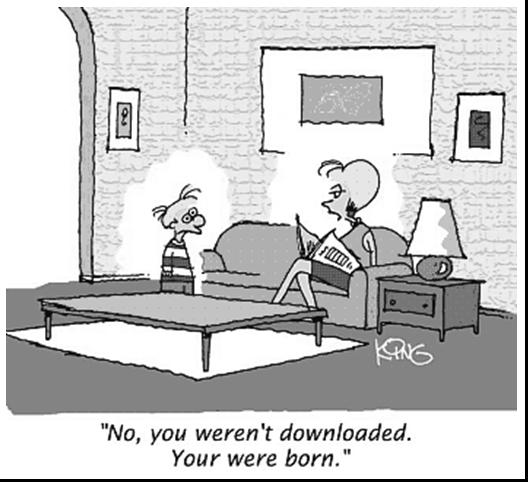
\includegraphics[width=.4\textwidth]{conteudo/figs/fig1.jpg}
    \fonte{\citeonline{SBC2024}}
\end{figure}

\begin{table}[!h]
    \centering
    \caption{Exemplo de Tabela}\label{tb:exemplo_tabela}
    \begin{tabular}{cccc}
        \hline Página & Topo & Baixo & Esquerda/Direita \\\hline
        Primeira & 3,5 & 2,5 & 1,5 \\
        Demais & 2,5 & 2,5 & 1,5 \\ \hline
    \end{tabular}
    \vspace{0.1cm}
    \fonte{Autoria própria (2024)}
\end{table}

\newpage

\begin{quadro}[!h]
    \centering
    \caption{Exemplo de Quadro}\label{tb:exemplo_quadro}
    \begin{tabular}{|c|c|c|c|}
        \hline Página & Topo & Baixo & Esquerda/Direita \\\hline
        Primeira & 3,5 & 2,5 & 1,5 \\ \hline
        Demais & 2,5 & 2,5 & 1,5 \\ \hline
    \end{tabular}
    \vspace{0.1cm}
    \fonte{Autoria própria (2024)}
    \vspace{0.1cm}
    \nota{Lorem ipsum dolor sit amet, consectetur adipiscing elit. Aenean ac viverra urna. Pellentesque vulputate erat vitae suscipit finibus. Vestibulum efficitur turpis vitae tincidunt cursus.}
\end{quadro}

\begin{codigo}[!h]
    \centering
    \caption{Exemplo de Código Fonte em Java}\label{cod:exemplo}
\begin{lstlisting}[language=Java]
public class Exemplo{
    public static void main(String[] args){
        System.out.println("Hello World!");
    }
}
\end{lstlisting}
    \fonte{Autoria própria (2024)}
\end{codigo}

\begin{algoritmo}[!h]
    \centering
    \caption{Método de Ordenação \textit{Bubble Sort}}\label{alg:exemplo}
    \begin{algorithm}[H]
        \SetAlgoBlockMarkers{início}{fim}
        \Dados{$vetor$, conjunto de dados a ser ordenado.}
        \Resultado{$vetor$, conjunto de dados ordenados após a execução do método.}
        \SetKwProg{Fn}{Função}{}{}\SetKwFunction{MetodoBolha}{metodoBolha}
        \SetKwFunction{TamanhoVetor}{obterTamanho}
        \AlgoDisplayBlockMarkers
    	\Fn{\MetodoBolha{vetor}}{
            \Para{inteiro i = 1 \Ate \TamanhoVetor{vetor} - 1}{
                \Para{inteiro j = 1 \Ate \TamanhoVetor{vetor} - i}{
                    \Se{vetor[j] $>$ vetor[j + 1]}{
                        inteiro temp = vetor[j] \\
                        vetor[j] = vetor[j + 1] \\
                        vetor[j + 1] = temp \\
                    }
                }
            }
            \Retorna{vetor}
    	}
    \end{algorithm}
    \fonte{Autoria própria (2024)}
\end{algoritmo}

\newpage

    % Referências.
    \referencias{referencias}

    % Espaço de Assinaturas.
    \assinaturas
\end{document}